\chapter{Automi a stati finiti}



\section{Automi a stati finiti deterministici (ASFD)}
Gli automi a stati finiti deterministici (ASFD) sono un moodello computazionale e rappresentano calcolatori semplici privi di memoria, ma viene solo memorizzato un registro contenente lo
stato interno, non è quindi possibile avere un contatore o qualsiasi altra variabile. L'\textbf{input} è sempre una stringa e l'\textbf{output} è un bit (0 o 1), serve quindi per problemi
di riconoscimento (vd. \ref{riconoscimento}). Come già accennato l'unica memoria di questi calcolatori è un registro che contiene lo \textbf{stato interno}.
Quindi, dato un input (una stringa) un ASFD esamina un simbolo della stringa alla volta e, dato che non c'è memoria esterna, non può riesaminare simboli precendenti.
L'\textbf{esecuzione} (spiegato in maniera informale) avviene in questo modo:
\begin{itemize}
    \item Viene esaminato il \textbf{simbolo corrente} della stringa e lo \textbf{stato interno corrente}
    \item Viene scelto se cambiare lo stato interno 
    \item Poi, se presente, si passa al simbolo successivo della stringa
    \item Arrivato alla fine della stringa la computazione termina e:
    \begin{itemize}
        \item Se lo stato interno corrente è uno \textbf{stato accettante}, viene restituito \textbf{1}
        \item Se lo stato interno corrente è uno \textbf{stato non accentante}, viene restituito \textbf{0}
    \end{itemize} 
\end{itemize}
Per rappresentare il funzionamento di una ASFD possiamo usare un \textbf{diagramma degli stati} (o \textbf{grafi di transizione}), eccone un esempio:
\begin{figure}[H]
    \centering  
    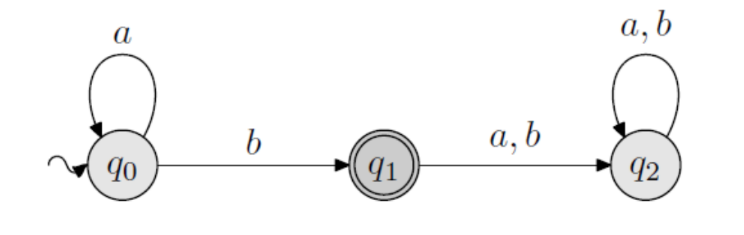
\includegraphics[width=0.8\linewidth]{../../images/grafo_trans.png}
    %\caption{caption}
    %\label{label}
\end{figure}
\noindent I \textbf{nodi} rappresentano i diversi stati e, se sono rappresentati con il doppio cerchio, sono stati accentati, altrimenti sono non accettanti. Gli \textbf{archi} rappresentano
le transizioni di stato, in pratica ci dice che se il simbolo è a, passo ad uno stato, e se il simbolo è b passa ad un altro stato.\smallskip\\
Compreso il funzionamento pratico di una ASFD, passiamo alle definizioni formali:\smallskip\\
\colorbox{SALZO}{\parbox{\dimexpr\linewidth-2\fboxsep}{\begin{definition}
   Un \textbf{automa a stati deterministici (ASFD)} è una quintupla $< \Sigma,Q,\delta,I,F  >$
\end{definition}}}\smallskip\\
Le componenti della quintupla sono:
\begin{itemize}
    \item $\mathbf{\Sigma}$: alfabeto (vd \ref{alfabeto}), è l'insieme dei possibili simboli utlizzati nelle stringhe (input).
    \item \textbf{Q}: insieme dei possibili stati interni $\{ q_0,q_1,\dots  \}$
    \item $\mathbf{I \in Q}$: stato iniziale dal quale parte la computazione
    \item $\mathbf{F \subseteq Q}$: Insieme degli stati accettanti
    \item $\mathbf{\delta: Q\times \Sigma \to Q}$: funzione di transizione, nel pratico è una tabella che indica lo stato successivo a seconda del simbolo analizzato 
\end{itemize}
Ecco un esempio:
